\documentclass[sigconf]{acmart}

\usepackage{booktabs} % For formal tables
\usepackage{siunitx}
\usepackage{color}

\newcommand{\comments}[1]{}
\newcommand{\xj}[1]{{\color{red}{xj:#1}}}

% Copyright
%\setcopyright{none}
%\setcopyright{acmcopyright}
%\setcopyright{acmlicensed}
\setcopyright{rightsretained}
%\setcopyright{usgov}
%\setcopyright{usgovmixed}
%\setcopyright{cagov}
%\setcopyright{cagovmixed}


% DOI
\acmDOI{10.475/123_4}

% ISBN
\acmISBN{123-4567-24-567/08/06}

%Conference
%\acmConference[WOODSTOCK'97]{ACM Woodstock conference}{July 1997}{El
%  Paso, Texas USA}
%\acmYear{1997}
%\copyrightyear{2016}


%\acmArticle{4}
%\acmPrice{15.00}

% These commands are optional
%\acmBooktitle{Transactions of the ACM Woodstock conference}
%\editor{Jennifer B. Sartor}
%\editor{Theo D'Hondt}
%\editor{Wolfgang De Meuter}


\begin{document}
\title{Room Layout Estimation from Multi-View Photos}
%\titlenote{Produces the permission block, and
%  copyright information}
%\subtitle{Extended Abstract}
%\subtitlenote{The full version of the author's guide is available as
%  \texttt{acmart.pdf} document}

\comments{
\author{Ruifeng Deng}
%\authornote{Dr.~Trovato insisted his name be first.}
\orcid{1234-5678-9012}
\affiliation{%
  \institution{University of Science and Technology of China}
  \streetaddress{P.O. Box 1212}
  \city{Hefei}
  \country{China}
  \postcode{43017-6221}
}
\email{trovato@corporation.com}

\author{Chaoyu Xie}
%\authornote{The secretary disavows any knowledge of this author's actions.}
\affiliation{%
  \institution{University of Science and Technology of China}
  \streetaddress{P.O. Box 1212}
  \city{Hefei}
  \country{China}
  \postcode{43017-6221}
}
\email{webmaster@marysville-ohio.com}

\author{Xuejin Chen}
%\authornote{This author is the
%  one who did all the really hard work.}
\affiliation{%
  \institution{University of Science and Technology of China}
  \streetaddress{1 Th{\o}rv{\"a}ld Circle}
  \city{Hefei}
  \country{China}}
\email{larst@affiliation.org}


% The default list of authors is too long for headers.
\renewcommand{\shortauthors}{B. Trovato et al.}
}

\begin{abstract}
Room layout estimation is a widely explored problem in indoor scene understanding. While most previous work focus on estimating the room layout in a single-view image, we try to extend the task using multi-view images. In this paper, we propose a simplified representation for room layout which is very easy to incorporate across views. A single-vew network (SVNet) is designed to learn the new representation. Given multi-view images, our system can estimate the combined room layout with large field of view which can even extend to the panorama. The results on real data look reasonable and impressive. We also achieve performance close to panorama based method on a panorama dataset.\footnote{This is an abstract footnote}
\end{abstract}

%
% The code below should be generated by the tool at
% http://dl.acm.org/ccs.cfm
% Please copy and paste the code instead of the example below.
%
\begin{CCSXML}
	<ccs2012>
	<concept>
	<concept_id>10010147.10010178.10010224.10010225.10010227</concept_id>
	<concept_desc>Computing methodologies~Scene understanding</concept_desc>
	<concept_significance>300</concept_significance>
	</concept>
	</ccs2012>
\end{CCSXML}

\ccsdesc[300]{Computing methodologies~Scene understanding}


\keywords{Scene understanding, Layout estimation, Object detection, Image stitching}


\maketitle

\section{Introduction}

\begin{figure*}
	\centering
	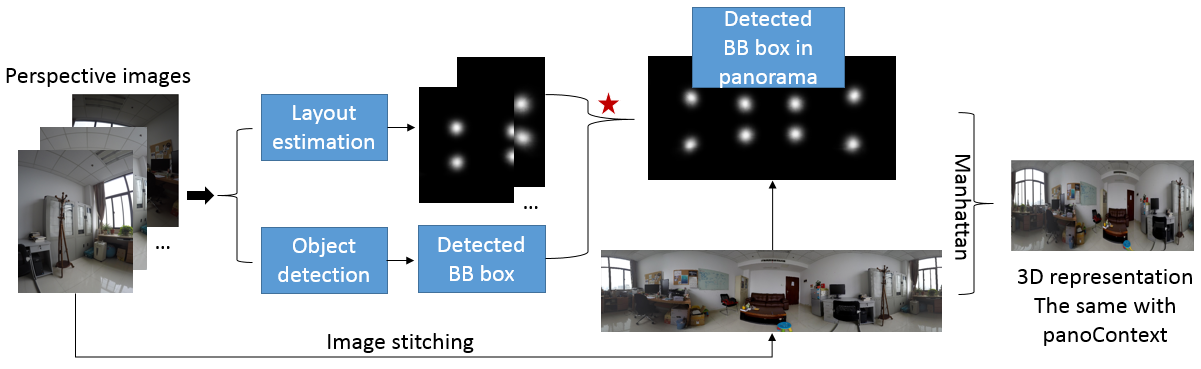
\includegraphics[width=\linewidth]{figs/ppline.png}
	\caption{Our pipeline consists of two main steps. First, a single-view network is employed to estimate the heatmap of room corners for each image separately. Secondly, the heatmaps of the input multi-view images are composed together to generate a combined heatmap of the room corners according to the image transformations. The final result is obtained by selecting the corners of local maximum.
		 }
	\label{fig:overview}
\end{figure*}

Indoor scene understanding has attracted wide attention due to its promising applications, including augmented/virtual reality and robotics. Massive researches have been carried out in related fields, such as semantic segmentation, room layout estimation and object detection. 
Room layout estimation is a fundamental task within scene understanding. It aims to predict the semantic boundaries between walls, the ceiling and the floor in a room. 
Since man-made indoor environments naturally follow some geometrical rules, for example objects always rest on the floor and many of them tend to be aligned with walls, the estimated room layout can provide valuable geometric priors, which can be applied in depth estimation, object detection~\cite{hedau2010thinking}, scene reconstruction \cite{lee2017joint} and so on.

%\xj{Traditional methods...}
Traditional approaches to this task usually follow a common proposing-ranking scheme \cite{hedau2009recovering,wang2013discriminative,gupta2010estimating,hedau2010thinking}. In the proposing stage, numerous layout hypotheses are obtained through vanishing point detection and ray sampling. Then, different hand-crafted features are used to find the best layout. 
\comments{
\xj{However, these techniques usually suffer from tedious and fragile post-processing tricks.}
\drf{It's the characteristic of DNN based method excluding \cite{zhao2017physics}}
}
With the rapid development of deep neural networks, recent methods built on fully convolutional network (FCN) have achieved remarkable performances in single-view images~\cite{mallya2015learning,dasgupta2016delay,ren2016coarse,zhao2017physics,LeeRoomNet17}. These networks efficiently learn object appearances and spatial distributions from a large database, and they implicitly encode these priors in the trained models to efficiently infer the layout of a new image. 
%\xj{limitations of single-view layout estimation techniques?}
%\xj{ambiguity of vertical walls, occluded corners.. multiple topology.}
%
However, these techniques usually suffer from tedious and fragile post-processing tricks. At the same time, single-view layout estimation has several inherent limitations, such as the ambiguity among walls claimed by \cite{dasgupta2016delay}, and the occlusion of critical semantic corners in a specific view. These limitations lead to non-perfect results that are still far from the requirements of practical applications.

%
While most of the previous work focused on estimating the room layout from one single-view image, we take more views into consideration. Unlike the single-view-based methods, the images taken from multi-views complement each other, which can ease the ambiguity caused by cluttered objects and occlusions of the room corners. At the same time, the combined room layout integrated from different views possess larger field of view (FOV) than that of the single-view layout. 
%
Few research has been carried out on multi-view-based layout estimation. \cite{bao2014understanding} follows the traditional proposing-ranking scheme in single-view layout estimation and merge the information from different views by integrating the structure from motion (SFM) into the framework. Their ranking part is implemented with complex hand-crafted features. 
%
In contrast, we propose a highly concise representation and an efficient algorithm to estimate the combined room layout from multi-view images.

%
Our work is similar in a sense to panorama-based room layout estimation \cite{zhang2014panocontext,zou2018layoutnet}. While we both explore a wider range of the room than a single shot, the panorama-based methods aim to recover the entire room structure in a \ang{360} panorama. 
%
\cite{zhang2014panocontext} presents a whole-room 3D context model which take a \ang{360} panorama as input and then outputs the detected objects and room layout. 
They extend the techniques used in single-view images by projecting the panorama into multiple perspective images first. 
In a subsequent technique \cite{zou2018layoutnet}, Zou et al. propose the LayoutNet network which are trained directly on panoramas to estimate the 3D room layout. They achieve better performance than \cite{zhang2014panocontext} in both accuracy and speed.
%
Inspired from these panorama-based methods, we design a new representation for room layout. Given multiple perspective images that are taken from different angles, we obtain a combined room layout at any FOV including the panoramic layout. Our approach also allows to revisit the same area several times because of the overlaps among multi-view images, which can enhance the prediction of interested space.

%
In order to reduce the ambiguities of different types of room layout, we propose a concise corner-based representation of room layouts in single-view image and design a single-view network to estimate these new corner-based layouts. 
The new representations of multiple views are easy to integrate.
We combine the estimated room layouts from different perspectives and generate a combined room layout using weighted average in the overlapping area. 
The final results look reasonable and impressive. 
We also evaluate our approach quantitatively on a panorama dataset and achieve comparable performance on whole-room layout with full \ang{360}-panorama-based methods without losing the flexibility.   

\comments{
To make full use of the contextual information for better understanding of an indoor scene, \cite{panocontext} present a whole-room 3D context model which take a \ang{360} panorama as input and then output the detected objects and room layout in 3D. They extends the techniques used in single-view images by projecting the panorama into multiple overlapping perspective images first. In a subsequent technique \cite{LayoutNet}, Zou et al. propose the LayoutNet network which trained directly on the panoramic images to estimate the 3D room layout. They achieve better performance in both accuracy and speed. However, it is not always convenient to obtain high-quality \ang{360} panoramic images that requires no position change between cameras in many applications. 
For this reason, we propose to explore the whole room structure using multi-view images \xj{that can be taken under different angles and locations} (if we know the camera position, yes) as an alternative scheme.

(add intro for multi-view layout estimation, there are two related papers using SFM) \xj{And compare our method with them.}
\xj{Emphasize our contribution and novelty here. }

By representing the entire room with multi-view images, we can naturally benefit from the mature techniques on perspective images. The estimated room layouts from different views can supplement each other and further improve the prediction accuracy of each perspective. Then we merge the prediction from multiple overlapping images and produce the holistic estimation of layout. The 3D structure of the entire room can be reconstructed from our holistic prediction, as depicted in Fig. \ref{fig:renderingResults}.
}



\section{Our Approach}
%\label{sec:approach}
Given multiple overlapping images of an indoor scene from different views, our approach produces the combined room layout represented by several room corners, as shown in Fig. \ref{fig:partial1}. When the overall FOV of the multi-view images contains the entire room, we can recover the whole-room layout, better viewed in panorama, Fig. \ref{fig:results2}. 
%
The algorithm pipeline is shown in Fig. \ref{fig:overview}. First, we estimate the partial room layout separately in each image using an encoder-decoder structure, as described in Sec. \ref{sec:layout}. Then the estimated partial room layouts are integrated into a combined probability map, based on the view transformations. 
We \xj{simply average?} use a linear blending to average the predictions from different views, and select the points of the maximum responses as the room corners, as described in Sec. \ref{sec:merging}. 

\comments{
We further align the panorama to be level with \xj{(what do you mean by be level with?)} the floor and reconstruct 3D structure of the room, as described in Sec.~\ref{sec:align}. 
}

\begin{figure*}[ht]
	\centering
	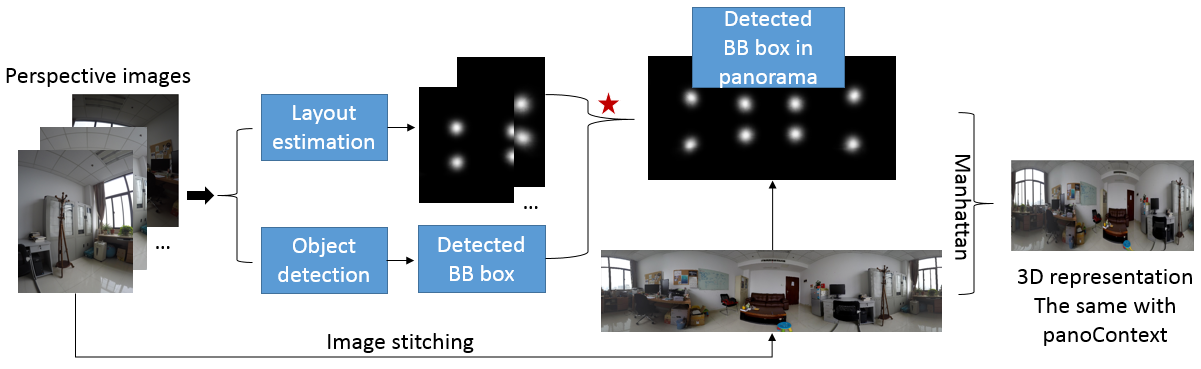
\includegraphics[width=\linewidth]{figs/ppline.png}
	\caption{Our pipeline consists of two main steps. Firstly, the SVNet is applied to estimate the probability map for each image seperately. Secondly, the multi-view images are aligned into a combined image using view transformation $f$. Then we use the same transformation $f$ to generate a combined probability map. The final result is obtained by a simple post-processing. }
	\label{fig:overview}
\end{figure*}

\subsection{Single-view room Layout Estimation}
\label{sec:layout}

Many methods have been proposed to estimate the room layout from a single RGB image. 
%In this section, we are going to recover the room layout for perspective images from different views. 
Previous DNN-based techniques of room layout estimation typically represent the room layout as a segmentation of semantic surfaces including walls, ceilings and floors~\cite{dasgupta2016delay, ours} or as the semantic boundaries or intersection points among them \cite{ren2016coarse}. 
%
These representations have proved valid and reasonable. However, due to the overlaps across views, they all carry too much redundant predictions and are inconvenient for combination under the circumstances of multi-view layout estimation. Out of this reason, we propose the \emph{secondary representation} of a room layout.
%
%A direct way to achieve our goal is to utilize existing methods to estimate the layout for each view, and then combine these representations to produce the complete-room 3D layout. 
%However, this method is not efficient due to many redundant predictions caused by overlaps across views. 
\comments{
To avoid redundant predictions or even to benefit from them, we propose a \emph{secondary representation} of a room layout on perspective images. The room layout under each view is only represented by the intersections of vertical walls and ceiling or floor. We call these intersections secondary keypoints. 
\xj{What about the case when there in only one wall surface?}
Obviously, without the extra intersections of two semantic planes on the image boundaries, we cannot recover the room layout from a single perspective. However, these secondary keypoints in overlapping views are sufficient to reconstruct the 3D layout of the entire room. Compared to previous representations, our secondary keypoints are quite simplified and easier to train. It also naturally avoids a lot of redundant predictions. 
}

\paragraph{Layout Representation.}
\xj{Explain more details of this new representation: add a figure. and more constraints? say, there are at most four points on each image? Split them to upper/lower parts?}
Under the Manhattan world assumption \cite{coughlan1999manhattan}, a 3D room can be modeled as a cube. The room layout in a single view is then the projection of this cube. As the cube can be defined by its 8 vertices, we adopt the location of these vertices, so called room corners, on the projected images to represent the room layout. Intuitively, there should be 0 to 4 room corners in a single-view image. 
%
Motivated by \cite{LeeRoomNet17} and the studies on human pose estimation \cite{tompson2014joint,pfister2015flowing}, we further formulate the room corners on the image plane as 2D Gaussian centered at their locations. The standard deviation is set to 40 pixels in our case.
%
Considering the inherent semantic differences, we classify the room corners into two categories: the upper room corner which is the intersection of two walls and ceiling, and the lower room corner which is the intersection of two walls and floor. In consequence, the goal of the single-view net should be estimating the probability maps of these two kinds of room corners for the input image, as depicted in Fig. \ref{fig:network}.
%
Compared to previous representations, our \emph{secondary representation} is quite simplified and easier to train. It also naturally avoids a lot of redundant predictions. 

 
%We use an encoder-decoder Network structure proposed in \cite{RoomNet} to estimate room layouts on perspective images. The room layout is represented by a series of keypoints in a particular order. The keypoints are the intersection of different semantic planes on the the perspective images. By learning the location of these keypoints, a room layout can be reconstructed by simply connect these keypoints in a specific order.

\noindent\textbf{Network Architecture.} We adopt the encoder-decoder architecture proposed by \cite{LeeRoomNet17} with modifications, \xj{since it is an end-to-end framework without any post-processing} since it can serve as an end-to-end framework that do not need complex post-processing. 
%
The modified network architecture, called SVNet, is shown in Fig.~\ref{fig:network}. It is designed to estimate the room corners in a single-view image. 
%Our network for room corner estimation from a single-view image is shown in Fig.~\ref{fig:network}.
\xj{We mainly make two modifications: decode part and classfication branch.} 
We mainly make two modifications: decode part and classfication branch. Firstly, as our secondary representation is easier to learn, we remove the recurrent structure in \cite{LeeRoomNet17} for efficiency, and then we add more upsampling layers and convolution layers to upsample the feature maps from the bottleneck layer to full input resolution as compensation for accuracy. The final convolution layer is adapted to output a $w \times h \times 2$ probability array $T$ for our new representation, where $w$ and $h$ stand for the width and length of the input image. Each of the 2 slices can be viewed as a probability map for the room corners in the corresponding category. Secondly, 
\cite{LeeRoomNet17} delineate room layout using 2D keypoints. The semantic boundaries can be recovered by connecting the detected 2D keypoints in a specific order. As the connection order differs between room topologies, they have to add a classification branch in their network to classify the room type, and the final performance rely on the classification accuracy. Unfortunately, the accuracy is not so well. We naturally avoid this awkward situation by using our \emph{secondary representation}. The simplified representation divides the room corners into only two categories and applies to all room types. So we elegantly remove the classification branch in our network architecture.

%First, the encoder part consists of 13 convolutional layers, which are topologically identical to the VGG16 network. It encodes the $320\times320$ input images to $10\times10$ feature maps. 
\comments{
We modify the decoder part to upsample the feature maps from the bottleneck layer with low resolution to full input resolution. \xj{what is the original decoder?}
%
Second, we remove the classification branch of the original RoomNet because our simplified representation is consist for different topology of visible surfaces in the scene. 
\xj{Therefore, our network outputs ... ?}
}

\begin{figure}
	\centering
	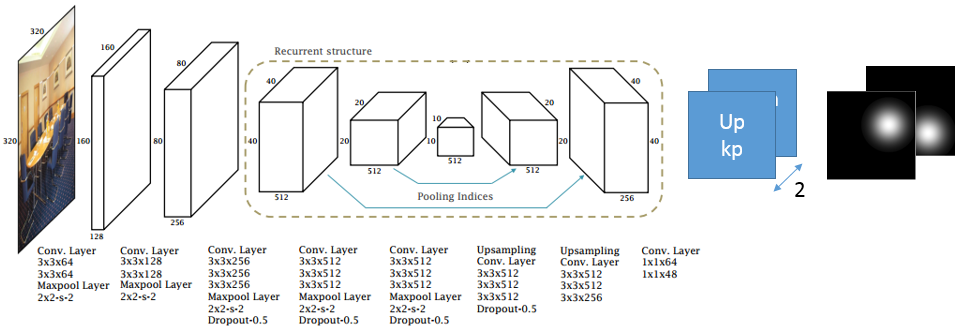
\includegraphics[width=\linewidth]{figs/network.png}
	\caption{Network architecture. The encoder part is topologically identical to the VGG16 network. It encodes the $320 \times 320$ input images to $10 \times 10$ feature maps. Then the decoder part upsample the feature maps from the bottleneck layer to full input resolution. }
	\label{fig:network}
\end{figure}

\noindent\textbf{Training.} 
We adopt the PanoContext dataset \cite{zhang2014panocontext} (and relabeled Stanford 2D-3D dataset \cite{layoutnet}) to generate multi-view images for training. The PanoContext dataset contains 500 annotated panoramic images. We project these panorama into multiple $320 \times 320$ images at different views using the toolkit provided by \cite{zhang2014panocontext}. The ground truth locations of the room corners are obtained using the same transformations and are further transformed into the Gausian representation. At training stage, Euclidean loss is used as the cost function to regress the probability map of room corners. As the area of the background is much larger than the foreground in the Gausian ground truth, we adjust the distribution imbalance between foreground and background pixels by degrading the gradient weight of background pixels with a coefficient of 0.2.

%To obtain multiple overlapping perspective images, we project the panoramic images into different views using the toolkit provided by \cite{pano}. The ground truth of the secondary keypoints is represented by several 2D Gaussian heatmaps centered at their locations. We adjust the distribution imbalance between foreground and background pixels by degrading the gradient weight of background pixels with a coefficient of 0.2.

%The RoomNet-basic struture in \cite{RoomNet} is adopted in our training stage for efficiency. We first pretrain the Network on LSUN \cite{LSUN2016} training set. Then, to finetune the model on images from different views in the same room, we project the panorama from \cite{PanoContext} to $k$ views. We set $k$ to 12 and 24 in our experiment. The layout ground truth is relabeled using the same projection. 

%The secondary keypoints can be divided into two categories according to semantics: the intersection of two walls and ceiling or the intersection of two walls and floor.\xj{Move this sentence to the representation paragraph.}

%We train the network to regress these two kinds of keypoints separately in order to eliminate the ambiguity between them. For this reason, the output of our network is a $w \times h \times 2$ probability array $T$, where $w$ and $h$ stand for the width and length of the input image. Each of the 2 slices can be viewed as a probability map for the secondary keypoints in a corresponding category. 


\subsection{Layout composition}
\label{sec:merging}
In this section, we composite the predicted layouts from different perspectives and generate a combined layout estimation. First, the input multi-view images are projected into a combined image using the camera poses, we formulate this view transformations as a function $f$. Then, we sum over the third dimension of the probability array $T$ for each image to get a heatmap $\hat{T}$ depicting all included room corners. Next, we use the same mapping $f$ to map the heatmap $\hat{T}$ from different views into a combined predictions. A linear blending along horizontal lines is applied to average the predictions of the overlapping area between different views, as shown in Fig. \ref{fig:blending}. 

%
After that, what we are going to do is picking the points of the maximum responses as the room corners. At this stage, we first reduce the noise in $\hat{T}$ caused by unsatisfactory predictions from particular perspectives. We calculate the LOG response of $\hat{T}$ at a certain scale (depending on the radius of the room corners), $\sigma$ is set to 21 in our case, and use the LOG response as our new heatmap.
%
Then, we follow the post-processing method in \cite{zou2018layoutnet} to obtain the locations of the room corners in the combined heatmap. In brief, the combined heatmap is summed across rows to find $m$ local maxima for columns, then $n$ largest peaks are found along each of the $m$ columns. In this way, we attain the locations of $m \times n$ room corners. In the case of panorama, $m$ is set to 4 and $n$ is set to 2. The whole room layout can be reconstructed by connecting these eight keypoints. 

\begin{figure}
	\centering
	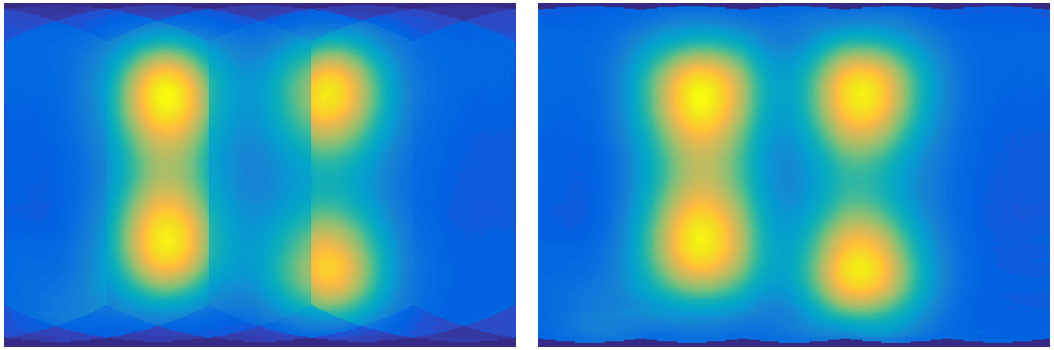
\includegraphics[width=\linewidth]{figs/blending.png}
	\caption{The combined probability map. Using simply average (left) or linear blending along horizontal lines (right).}
	\label{fig:blending}
\end{figure}


\comments{
\subsection{Alignment and 3D Reconstruction}
\label{sec:align}

(Optional and undone) In this section, we align the panoramic images to make sure that wall-wall boundaries are vertical to the floor. If we use the panorama to generate testing images, this step can be omitted as the reprojected panoramic images naturally met this alignment condition. Then the aligned panorama can be further rendered into a 3D representation. These two steps are implemented using existing techniques but the rendering part is not yet available. 
}



\section{Results}
Our approach performs well on real data even facing occlusions and clutter in the indoor enviroment. A panoramic visual sample taken from the PanoContext testset is shown in Fig. \ref{fig:results2}.
%
The first row are the input multi-view images, the second row are the predicted probability maps from the network. We also estimate the room corners on the flipped version of the input images and average the corresponding probability maps. Then the predictions from different views are merged to generate the overall probability map on the left of the third row, and the final result is on its right. 
%
In this scene, 12 images from different horizontal perspectives are used. Note that several room corners are occluded by objects, such as the corners behind the bed and the sofa, but we can still recover the overall layout of the room properly. As revealed by the probability maps, the uncertainty of the lower room corner in the second view has been compensated by the first view. Our method also show robustness to complex texture, such as patterned carpet in this scene. 
%
Fig. \ref{fig:partial2} shows a combined layout generated by 4 perspective images. Our method works well in this situation too. The SVNet correctly infer the layout without room corners, as depicted in the second view, and it is robust to clutter caused by many objects around the lower room corners.


\begin{figure}[ht]
	\centering
	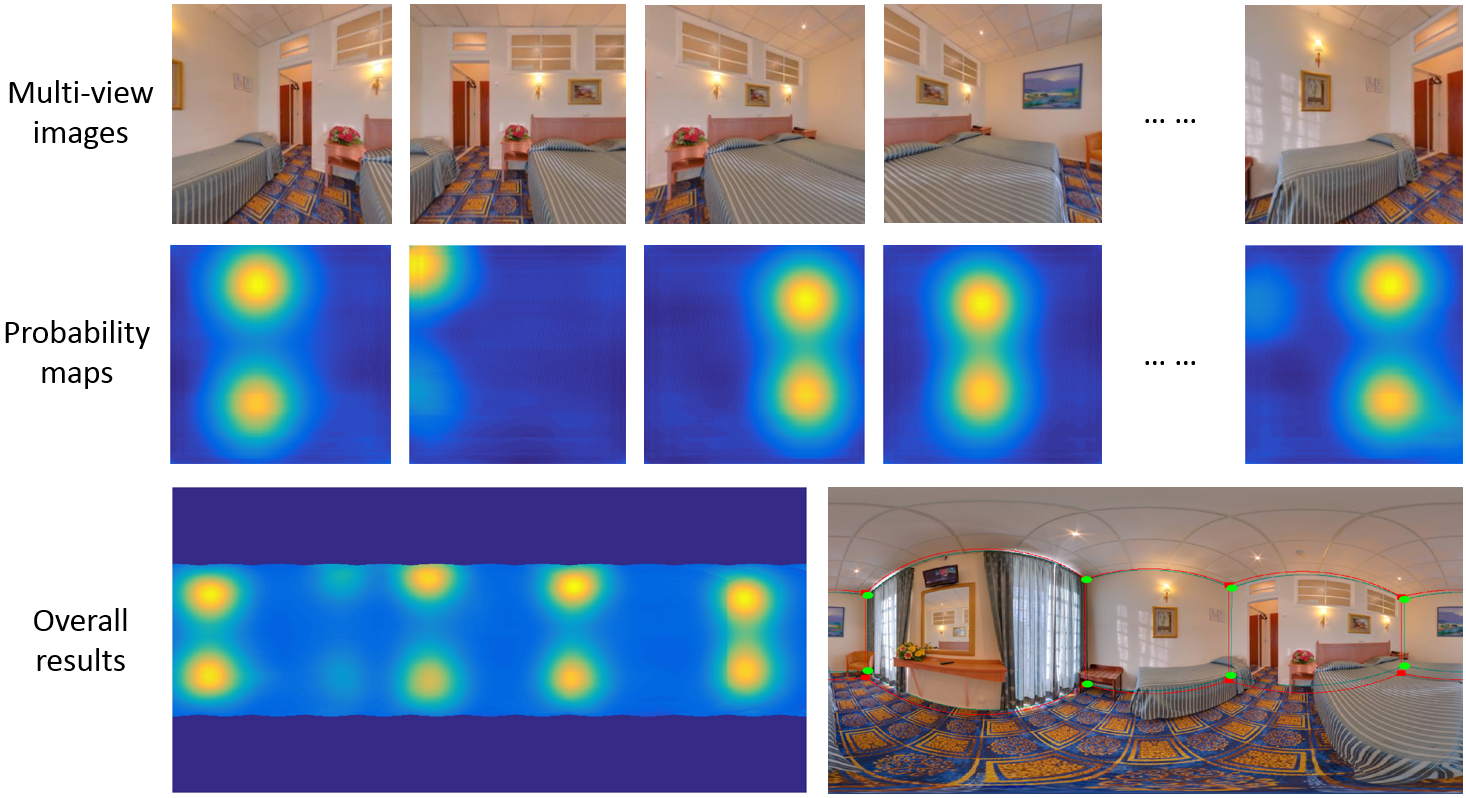
\includegraphics[width=\linewidth]{figs/results2.png}
	\caption{Our qualitative results on real data. We sum over the third dimension of the probability array $T$ for visulization. In the final result, the ground truth is shown in green and our prediction is shown in red. }
	\label{fig:results2}
\end{figure}

\begin{figure}
	\centering
	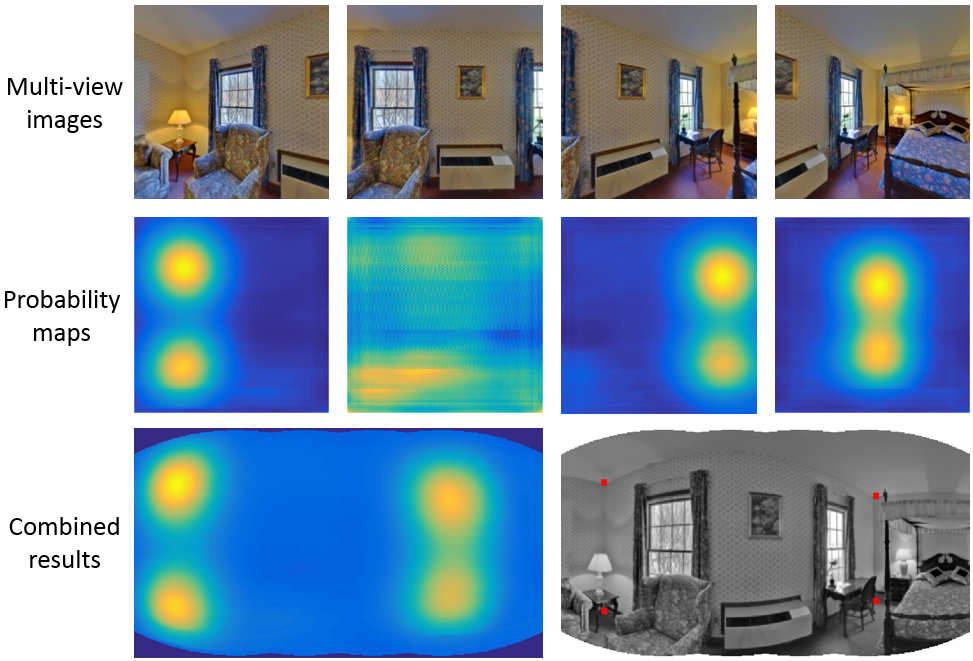
\includegraphics[width=\linewidth]{figs/partial2.png}
	\caption{A combined layout generated from four images. The predicted room corners are depicted by red points in the final result.}
	\label{fig:partial2}
\end{figure}


We also conduct experiments on the PanoContext dataset for quantitive comparison with previous panorama based methods, the same training/testing split is adopted. 
%
Three standard metrics are adopted for evaluation: 3D Intersection over Union, Corner error and Pixel error. As shown in Tab. \ref{tab:PC}, our approach is nearly on par with the panorama based methods. 
%
We believe that the reason for this deficiency is that the FOV of each perspective image is much smaller than that of the panorama. Limited FOV may lead to the wrong focus, which then pollutes the overall prediction. 
%
To explore the effect of using different size of FOV, we use two different settings during training and testing. For Multi-view-\ang{60}, we project the panorama into 24 perspective images with $FOV=\ang{60}$, while 8 directions around the vertical axis and 3 directions around the horizontal axis. For Multi-view-\ang{90}, we project the panorama into 12 perspective images with $FOV=\ang{90}$, all of them are horizontal and centered around the vertical axis. 
%
The quantitative results in Tab. \ref{tab:PC} demonstrate that larger FOV contribute to higher accuracy in overall prediction, which is also consistent with our intuition. In fact, the panorama can be viewed as a special case that the FOV reaches its maximum.


%Experiments, three parts: one for different field of view (FOV), one for comparison with panorama based method, the last one for qualitative results.


%\begin{table}
%	\caption{Results of different FOV.}
%	\label{tab:FOV}
%	\begin{tabular}{cccc}
%		\toprule
%		FOV &3D IoU (\%)&Corner error (\%)&Pixel error (\%)\\
%		\midrule
%		 \ang{60} & XX & XX & XX\\
%	     \ang{90} & XX & XX & XX\\	
%		\bottomrule
%	\end{tabular}
%\end{table}


\begin{table}
	\caption{Quantitative results on PanoContext dataset. \drf{the fourth row is the result for \ang{90} without estimating the flipped verison and average. Not sure if it should be removed.}}
	\label{tab:PC}
	\begin{tabular}{cccc}
		\toprule
		Method&3D IoU (\%)& $\epsilon_{corner}$ (\%) & $\epsilon_{pixel}$ (\%)\\
		\midrule
		PanoContext \cite{zhang2014panocontext} & 67.23 & 1.60 & 4.55\\
		LayoutNet \cite{zou2018layoutnet} & 74.48 & 1.06 & 3.34\\
		Multi-view-\ang{60} & 53.39 & 3.35 & XX\\	
		\ang{90} & 59.58 & \textbf{2.20} & 6.78\\	
		Multi-view-\ang{90} & \textbf{61.98} & 2.75 & \textbf{6.73}\\	
		\bottomrule
	\end{tabular}
\end{table}

\section{Conclusions}
In this paper, we propose a method to estimate the combined room layout based on multiple views. We design a concise representation for the room layout in the perspective image to simplify the learning process. Then we integrate the predicted room layout from different perpectives into a combined prediction using view transformations and a fusion strategy. The multi-view images can supplement each other and generate more accurate predicitons. We also achieve performance close to the panorama based methods on a panorama dataset. It is an encouraging attempt to estimate the room layout with larger FOV using multi-view images.

\comments{
\begin{acks}
	The authors would like to thank ...
\end{acks}
}

\comments{
\begin{figure}
	\centering
	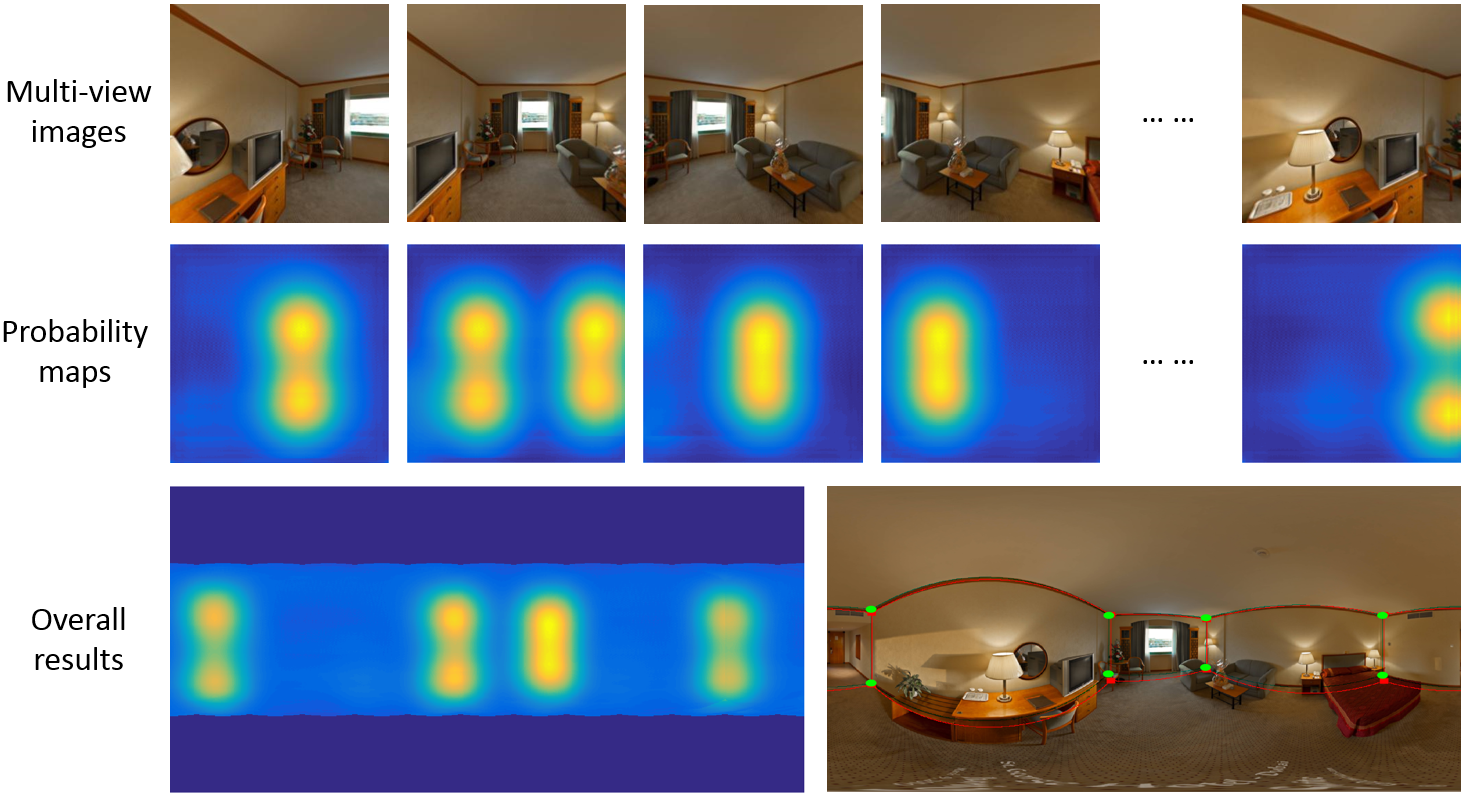
\includegraphics[width=\linewidth]{figs/results3.png}
	\caption{alternative/more results. }
	\label{fig:results3}
\end{figure}

\begin{figure}
	\centering
	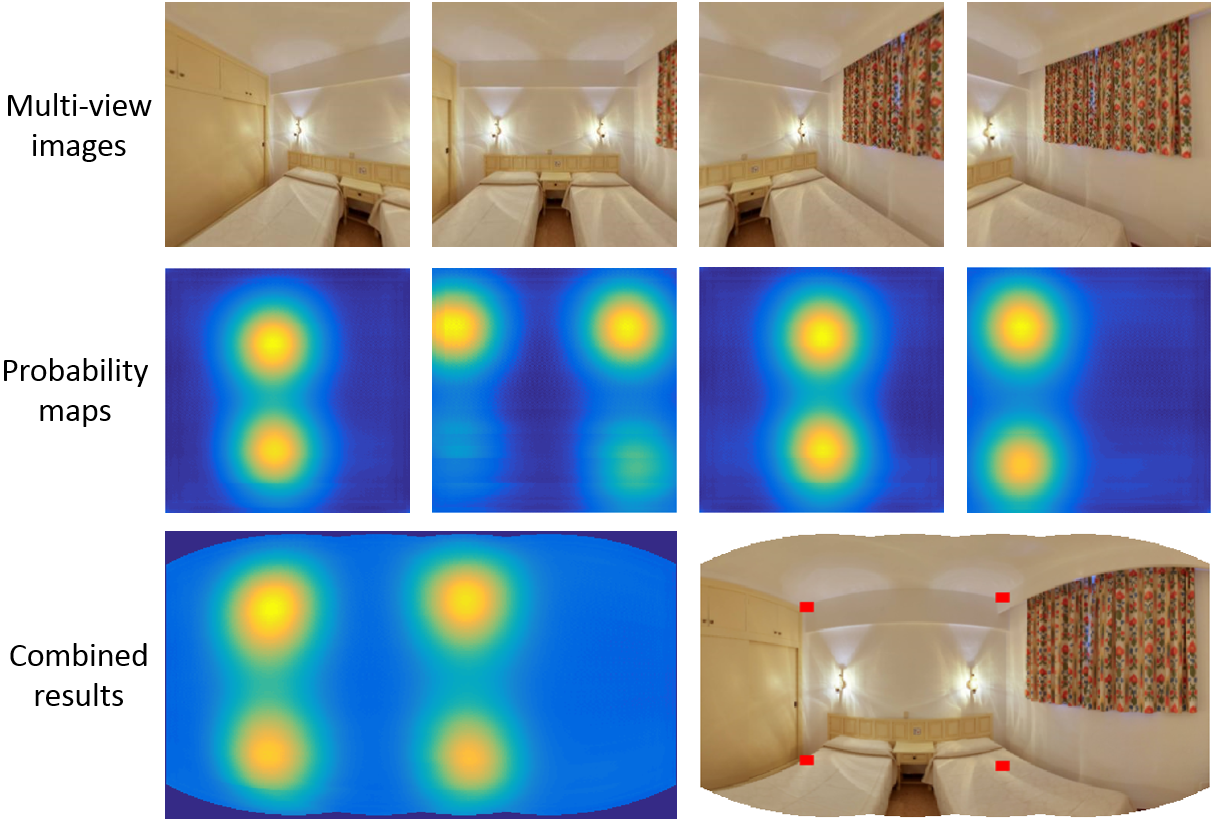
\includegraphics[width=\linewidth]{figs/partial1.png}
	\caption{alternative/more results for combined partial views. }
	\label{fig:partial1}
\end{figure}
}
%\section{Introduction}

In recent years, indoor scene understanding has attracted wide attention due to its promising applications, including augmented/virtual reality and robotics. Massive researches have been carried out in related fields, such as semantic segmentation, room layout estimation and object detection. However, most of the previous work focused on solving the above problems with 2D images from a single perspective. The scenario information from a single view is quite limited and difficult to meet the requirements of practical high-level applications. In this paper, we try to explore the whole layout of an indoor scene using multi-view images.

Room layout estimation is a fundamental task within scene understanding. It aims to predict semantic boundaries among walls, ceiling and floor. Due to the development of deep neural networks, recent methods built on FCN have achieved remarkable performance in single-view images \cite{PIO,CFILE,DELAY,ICIP2018}. To make full use of contextual information for better understanding of an indoor scene, \cite{panocontext} present a whole-room 3D context model which take a \ang{360} panorama as input and then output the detected objects and room layout in 3D. They extends the techniques used in single-view images by projecting the panorama into multiple overlapping perspective images first. In a subsequent technique \cite{LayoutNet}, Zou et al. propose the LayoutNet network which trained directly on the panoramic image to estimate the 3D room layout. They achieve better performance in both accuracy and speed. However, it's not always convenient to obtain high-quality \ang{360} panoramic images in practical application. For this reason, we propose to explore the whole room structure using multi-view images as an alternative scheme.


By representing the entire room with multi-view images, we can naturally benefit from the mature techniques on perspective images. The estimated room layouts from different views can supplement each other and further improve the prediction accuracy of each perspective. Then we merge the prediction from multiple overlapping images and produce the holistic estimation of layout. The 3D structure of the entire room can be reconstructed from our holistic prediction, as depicted in Fig. \ref{fig:renderingResults}.

(add intro for multi-view layout estimation, there are two related papers using SFM) 

\section{Approach}
Given multiple images of an indoor scene from different views, our framework produces the corresponding whole-room layout estimation. Fig. \ref{fig:overview} shows the system overview. We first estimate the room layout seperately in multiple perspective images, details can be found in Sec. \ref{sec:layout}. Then the estimated room layouts are integrated into a panorama through image stitching. We average the prediction from different views to improve the overall accuracy, as described in Sec. \ref{sec:merging}. We further align the panorama to be level with the floor and reconstruct 3D structure of the room, as described in Sec. \ref{sec:align}. 

\begin{figure*}
	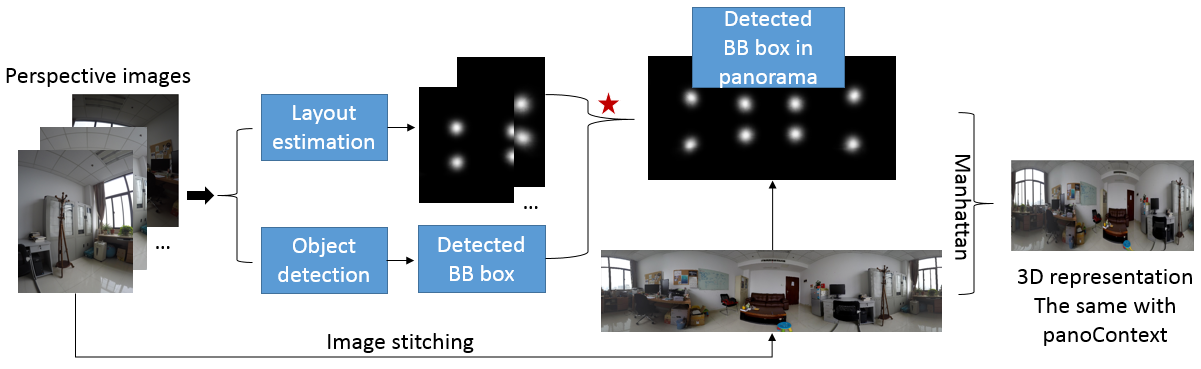
\includegraphics[height=2in, width=7in]{figs/ppline.png}
	\caption{System overview. (Need to be refined, and the image size will be normalized soon)}
	\label{fig:overview}
\end{figure*}

\subsection{Room Layout Estimation}
\label{sec:layout}
In this section, We are going to recover the room layout for perspective images from different views. Previous techniques of room layout estimation on perspective images typically represent the room layout as a segmentation of semantic surfaces including walls, ceilings and floors \cite{Delay,ours} or as the semantic boundaries or intersection points among them \cite{CFILE}. A direct way to achieve our goal is to utilize the existing methods to estimate the layout for each perspective, and then combine these representations to produce the whole-room 3D layout. However, this method is not efficient due to many redundant predictions caused by overlaps across views. To avoid redundant predictions or even to benefit from them, we propose a secondary representation of a room layout on perspective images. The room layout under each view is only represented by the intersections of two walls and ceiling or floor. We call these intersections secondary keypoints. Obviously, without the extra intersections of two semantic planes on the image boundaries, we cannot recover the room layout from a single perspective. However, these secondary keypoints in overlapping views are sufficient to reconstruct the 3D layout of the entire room. Compared to previous representations, our secondary keypoints are quite simplified and easier to train. It also naturally avoids a lot of redundant predictions. 
 
%We use an encoder-decoder Network structure proposed in \cite{RoomNet} to estimate room layouts on perspective images. The room layout is represented by a series of keypoints in a particular order. The keypoints are the intersection of different semantic planes on the the perspective images. By learning the location of these keypoints, a room layout can be reconstructed by simply connect these keypoints in a specific order.

\noindent\textbf{Network Architecture.} We adopt the encoder-decoder architecture proposed by \cite{roomnet} with modifications. As shown in Fig. \ref{fig:network}, the encoder part consists of 13 convolutional layers, which are topologically identical to the VGG16 network. It encodes the $320\times320$ input images to $10\times10$ feature maps. Then we modify the decoder part to upsample the feature maps from the bottleneck layer with low resolution to full input resolution. As our simplified representation no longer depends on the topological category of the room, we further remove the classification branch. 

\begin{figure}
	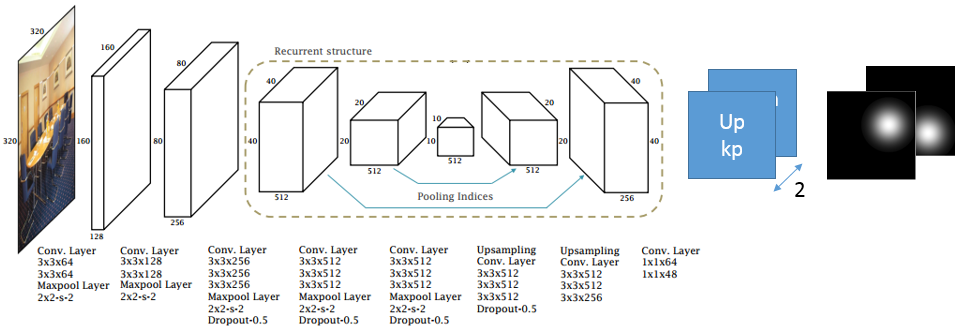
\includegraphics[height=1.5in, width=3in]{figs/network.png}
	\caption{Network architecture. (Need to be refined, and the image size will be normalized soon)}
	\label{fig:network}
\end{figure}

\noindent\textbf{Training.} The secondary keypoints can be divided into two categories according to semantics: the intersection of two walls and ceiling or the intersection of two walls and floor. We train the network to regress these two kinds of keypoints seperately in order to eliminate the ambiguity between them. For this reason, the output of our network is a $w \times h \times 2$ probability array $T$, where $w$ and $h$ stand for the width and length of the input image. Each of the 2 slices can be viewed as a probability map for the secondary keypoints in a corresponding category. We adopt the PanoContext dataset \cite{pano} and relabeled Stanford 2D-3D dataset \cite{layoutnet} to train our layout estimation network. To obtain multiple overlapping perspective images, we project the panoramic images into different views using the toolkit provided by \cite{pano}. The ground truth of the secondary keypoints is represented by several 2D Gaussian heatmaps centered at their locations. We adjust the distribution imbalance between foreground and background pixels by degrading the gradient weight of background pixels with a coefficient of 0.2.

%The RoomNet-basic struture in \cite{RoomNet} is adopted in our training stage for efficiency. We first pretrain the Network on LSUN \cite{LSUN2016} training set. Then, to finetune the model on images from different views in the same room, we project the panorama from \cite{PanoContext} to $k$ views. We set $k$ to 12 and 24 in our experiment. The layout ground truth is relabeled using the same projection. 


\subsection{Generation of Panorama}
\label{sec:merging}
In this section, we combine the predicted layouts from different perspectives and generate a panoramic layout estimation. Fisrt, we stitch the input multi-view images into a panoramic image. Then, we use the same mapping to map the predicted probability array $T$ from different views into a panoramic predictions and averaged across views. To reduce the noise caused by false predictions from specific perspectives, we calculate the LOG response of the panoramic predictions at a certain scale (depending on the radius of the keypoints), $\sigma$ is set to 21 in our case. After that, we sum up the probability maps from two channel to get a holistc probability map. Finally, we follow the post-processing method in \cite{LayoutNet} to obtain the locations of the keypoints in the panorama. In brief, the holistic probability map are summed across rows to find four local maxima for columns, then two largest peaks are found along each of the four columns. In this way, we attain the location of eight keypoints for each panorama. Then the whole room layout can be reconstructed by connecting these eight keypoints. 


\subsection{Alignment and 3D Reconstruction}
\label{sec:align}

(Optional and undone) In this section, we align the panoramic images to make sure that wall-wall boundaries are vertical to the floor. If we use the panorama to generate testing images, this step can be omitted as the reprojected panoramic images naturally met this alignment condition. Then the aligned panorama can be further rendered into a 3D representation. These two steps are implemented using existing techniques but the rendering part is not yet available. 


\section{Results}
Our approach performs well on real data even facing occlusions and clutter in the indoor enviroment. A visual sample is shown in Fig. \ref{fig:results1}. The first row are the input multi-view images, the second row are the predicted probability maps from the network. We do the same prediction on the flipped version of the input images and average the corresponding probability maps. Then the predictions from different views are merged to generate the overall probability map on the left of the third row, and the final result is on its right. In this scene, 12 images from different horizontal perspectives are used. Note that several secondary keypoints are occluded by objects, such as the keypoints behind the bed and the TV, but we can still recover the overall layout of the room properly. Our method also show robustness to clutter, such as the many small objects around the TV. (maybe more visual results and analysis)

\begin{figure}
	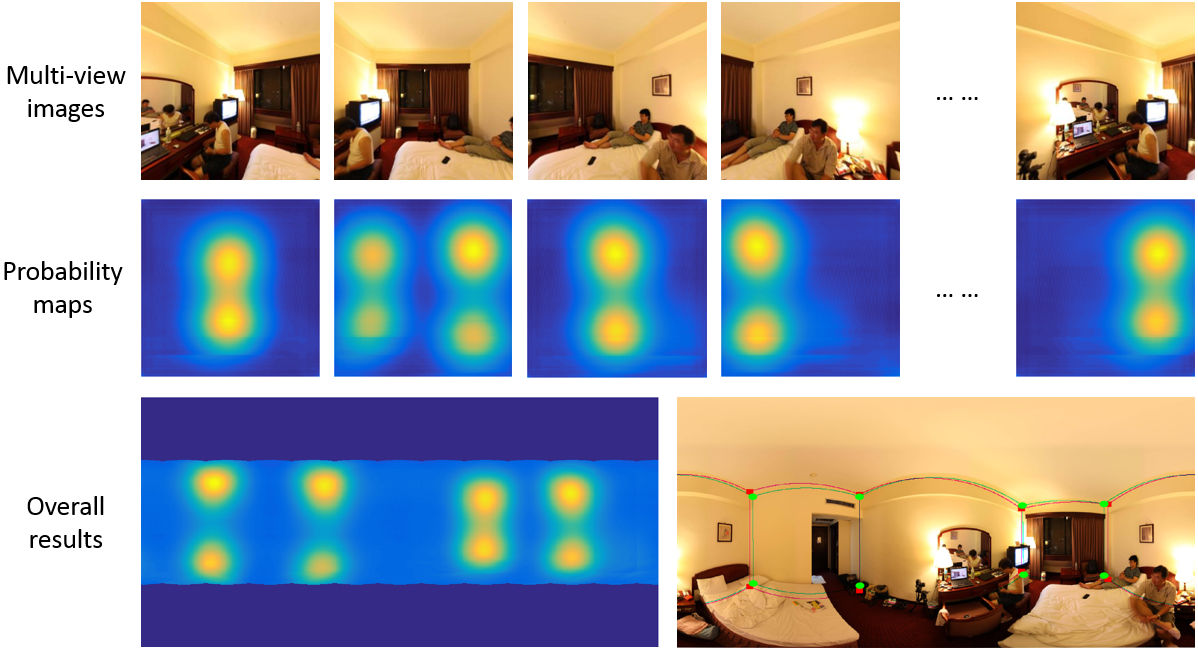
\includegraphics[height=1.5in, width=3in]{figs/results1.png}
	\caption{Our qualitative results on real data. We sum over the third dimension of the probability array $T$ for visulization. In the final result, the ground truth is shown in green and our prediction is shown in red. (Need to be refined, and the image size will be normalized soon)}
	\label{fig:results1}
\end{figure}

We also conduct experiments on the PanoContext testset for quantitive comparison with previous panorama based methods. Three standard metrics are adopted for evaluation: 3D Intersection over Union, Corner error and Pixel error. As shown in Tab. \ref{tab:PC}, our approach is nearly on par with the panorama based methods. We believe that the reason for this deficiency is that the FOV of each perspective image is much smaller than that of the panorama. Limited FOV may lead to the wrong focus, as shown in Fig. \ref{wrong}, which then pollutes the overall prediction. To explore the effect of using different size of FOV, we use two different settings during training and testing. For \ang{60}, we project the panorama into 24 perspective images with $FOV=\ang{60}$, while 8 directions around the vertical axis and 3 directions around the horizontal axis. For \ang{90}, we project the panorama into 12 perspective images with $FOV=\ang{90}$, all of them are horizontal and centered around the vertical axis. The quantitative results in Tab. \ref{tab:PC} demonstrate that larger FOV contribute to higher accuracy in overall prediction, which is also consistent with our intuition. In fact, the panorama can be viewed as a special case that the FOV reaches its maximum.


%Experiments, three parts: one for different field of view (FOV), one for comparison with panorama based method, the last one for qualitative results.


%\begin{table}
%	\caption{Results of different FOV.}
%	\label{tab:FOV}
%	\begin{tabular}{cccc}
%		\toprule
%		FOV &3D IoU (\%)&Corner error (\%)&Pixel error (\%)\\
%		\midrule
%		 \ang{60} & XX & XX & XX\\
%	     \ang{90} & XX & XX & XX\\	
%		\bottomrule
%	\end{tabular}
%\end{table}


\begin{table}
	\caption{Quantitative results on PanoContext dataset.}
	\label{tab:PC}
	\begin{tabular}{cccc}
		\toprule
		Method&3D IoU (\%)&Corner error (\%)&Pixel error (\%)\\
		\midrule
		PanoContext & 67.23 & 1.60 & 4.55\\
		LayoutNet & 74.48 & 1.06 & 3.34\\
		Our Method \ang{60} & XX & XX & XX\\	
		Our Method \ang{90} & 59.58 & 2.20 & 6.78\\	
		\ang{90} add flip & 61.98 & 2.75 & 6.73\\	
		\bottomrule
	\end{tabular}
\end{table}

\section{Conclusions}
In this paper, we propose a method to estimate the overall room layout based on multiple views. We design a secondary representation for the room layout in the perspective image to simplify the learning process. Then we integrate the predicted room layout from different perpectives into a holistic prediction using image stitching and a fusion strategy. Our output panoramic results can be further rendered into a 3D representation. This is an encouraging attempt to estimate the whole room layout using multiple perspectives and without using structure from motion.


\begin{acks}
  The authors would like to thank ...
\end{acks}


\bibliographystyle{ACM-Reference-Format}
\bibliography{sample-bibliography}

\end{document}
